% rel_chapter_13_sec120.tex
% Agent 58: Relativistic Jeans instability with rotation and magnetic field (Ch XIII §120)
% Conventions: (-,+,+,+) signature, c kept explicit, see RELATIVISTIC_CONVENTIONS.md

\section{Effects of Rotation and Magnetic Field on the Relativistic Jeans Criterion}
\label{sec:rel-120}

In the classical treatment (\S\,120), Chandrasekhar proved that
Jeans's criterion for gravitational instability of an infinite
homogeneous medium is \emph{unaffected} by the separate or simultaneous
presence of a uniform rotation and a uniform magnetic field.  The
physical content of that theorem carries over to the relativistic
regime, but its quantitative expression is modified in several important
respects:
\begin{enumerate}
\item[(i)] The rest-mass density~$\rho$ is replaced, wherever inertia
  enters, by the relativistic enthalpy density
  $\enthalpy = (\varepsilon + p)/c^{2}$, where $\varepsilon$ is the
  total energy density (rest mass $+$ internal energy) and $p$ is the
  pressure.
\item[(ii)] The sound speed $\cs$ must satisfy the causality bound
  $\cs^{2} = (\partial p/\partial\varepsilon)_{s} \le c^{2}$.
\item[(iii)] The Alfv\'en speed is bounded above by~$c$ and takes the
  relativistic form
  $\vA^{2} = b^{2}/(4\pi\enthalpy + b^{2})\,c^{2}$, where
  $b^{2} = b^{\mu}b_{\mu}$ is the covariant magnetic pressure
  parameter.
\item[(iv)] All characteristic wave speeds (sound, Alfv\'en, fast and
  slow magnetosonic) must individually satisfy $v \le c$; this
  constrains the allowed parameter space and ensures causal propagation
  of every perturbation mode.
\item[(v)] Gravitational effects are encoded through a relativistic
  Poisson-like equation deriving from the linearised Einstein equations
  in the weak-field limit, with source $\varepsilon + 3p$ rather than
  $\rho$ alone.
\end{enumerate}

\noindent
We develop the relativistic extensions in the same three stages as in
the classical analysis: rotation alone, magnetic field alone, and the
two combined.

%------------------------------------------------------------------
\subsection*{(a) \textit{Rotation: relativistic dispersion with Coriolis
  force}}
\label{subsec:rel-120a}

\subsubsection*{Setup and linearised equations}

Consider an infinite homogeneous relativistic perfect fluid with
equilibrium enthalpy density $\enthalpy_{0}$, energy density
$\varepsilon_{0}$, pressure~$p_{0}$, and sound speed~$\cs$.  The fluid
rotates uniformly with angular velocity~$\boldsymbol{\Omega}$.  In a
frame corotating with~$\boldsymbol{\Omega}$, the Coriolis acceleration
takes the same kinematic form as in Newtonian theory, but the inertia
of the fluid element is set by $\enthalpy_{0}$ rather than $\rho_{0}$.
The linearised relativistic Euler equation in the corotating frame is
\begin{equation}
  \enthalpy_{0}\,\frac{\partial\mathbf{u}}{\partial t}
  = -\operatorname{grad}\delta p
    + \enthalpy_{0}\,\operatorname{grad}\delta\mathfrak{B}
    + 2\,\enthalpy_{0}\,\mathbf{u}\times\boldsymbol{\Omega}\,,
  \label{eq:rel13-90}
\end{equation}
where $\mathbf{u}$ is the Eulerian velocity perturbation and
$\delta\mathfrak{B}$ is the perturbation in the gravitational
potential.  The relativistic continuity equation (conservation of
baryon number, or equivalently of energy in the isentropic case) and the
relativistic Poisson equation read
\begin{equation}
  \frac{\partial}{\partial t}\delta\varepsilon
  + (\varepsilon_{0}+p_{0})\,\operatorname{div}\mathbf{u} = 0\,,
  \label{eq:rel13-91}
\end{equation}
\begin{equation}
  \nabla^{2}\delta\mathfrak{B}
  = -4\pi G\bigl(\delta\varepsilon + 3\,\delta p\bigr)
  = -4\pi G\bigl(1 + 3\cs^{2}/c^{2}\bigr)\delta\varepsilon\,.
  \label{eq:rel13-92}
\end{equation}
Note that the factor $(1 + 3\cs^{2}/c^{2})$ on the right-hand side of
the Poisson equation encodes the relativistic enhancement of the
gravitational source: pressure contributes to gravity in general
relativity.  In the Newtonian limit $\cs^{2}/c^{2}\to 0$ and
$\enthalpy_{0}\to\rho_{0}$, equations
\eqref{eq:rel13-90}--\eqref{eq:rel13-92} reduce to the classical
system~\eqref{eq:13-90}, \eqref{eq:13-95}, \eqref{eq:13-96}.

\subsubsection*{Dispersion relation}

We seek plane-wave perturbations proportional to
$\exp[i(kz + \sigma t)]$, with $\boldsymbol{\Omega}$ inclined at
angle~$\vartheta$ to the direction of propagation.  Following the same
algebraic reduction as in the classical case (expanding the determinant
of the resulting linear system), we obtain the relativistic
characteristic equation
\begin{equation}
\boxed{
  \sigma^{4}
  - \Bigl(4\Omega^{2} + \cs^{2}k^{2}
    - 4\pi G\,\enthalpy_{0}\bigl(1+3\cs^{2}/c^{2}\bigr)
    \Bigr)\,\sigma^{2}
  + 4\Omega^{2}\Bigl(\cs^{2}k^{2}
    - 4\pi G\,\enthalpy_{0}\bigl(1+3\cs^{2}/c^{2}\bigr)
    \Bigr)\cos^{2}\!\vartheta
  = 0\,.}
  \label{eq:rel13-99}
\end{equation}
This is the direct relativistic generalisation of the classical
equation~\eqref{eq:13-99}.  The two modifications are:
\begin{enumerate}
\item[(i)] The effective gravitational coupling is enhanced:
  $4\pi G\rho \to 4\pi G\,\enthalpy_{0}(1+3\cs^{2}/c^{2})$, because
  both the enthalpy (inertial + gravitational mass) and the pressure
  serve as gravitational sources.
\item[(ii)] The sound speed $\cs$ is bounded by causality,
  $\cs \le c$.
\end{enumerate}

\subsubsection*{Modified Jeans criterion}

The condition for gravitational instability is that the product
$\sigma_{1}^{2}\sigma_{2}^{2} < 0$, which from
equation~\eqref{eq:rel13-99} requires
\begin{equation}
  \cs^{2}\,k^{2}
  < 4\pi G\,\enthalpy_{0}\bigl(1 + 3\cs^{2}/c^{2}\bigr)\,.
  \label{eq:rel13-jeans-rot}
\end{equation}
The relativistic Jeans wavenumber is therefore
\begin{equation}
  k_{\mathrm{J,rel}}^{2}
  = \frac{4\pi G\,\enthalpy_{0}}{\cs^{2}}
    \,\bigl(1 + 3\cs^{2}/c^{2}\bigr)\,,
  \label{eq:rel13-kJ}
\end{equation}
and the corresponding Jeans mass
\begin{equation}
  M_{\mathrm{J,rel}}
  = \frac{4\pi}{3}\,\enthalpy_{0}
    \left(\frac{\pi}{k_{\mathrm{J,rel}}}\right)^{3}
  = \frac{\pi^{5/2}\,\cs^{3}}{6\,G^{3/2}\,
    \enthalpy_{0}^{1/2}\,
    \bigl(1+3\cs^{2}/c^{2}\bigr)^{3/2}}\,.
  \label{eq:rel13-MJ}
\end{equation}
As in the classical theory, rotation does \emph{not} alter the Jeans
criterion itself---but it does stabilise the mode propagating
perpendicular to~$\boldsymbol{\Omega}$ ($\vartheta = \pi/2$) whenever
$\Omega^{2} > \pi G\,\enthalpy_{0}(1+3\cs^{2}/c^{2})$.

\subsubsection*{Relativistic Toomre parameter}

For a rotating, self-gravitating disc the local stability criterion is
conveniently expressed through the Toomre parameter.  In the
relativistic extension, the epicyclic frequency~$\kappa$ and the
surface density~$\Sigma$ must be computed from the relativistic
equilibrium.  Writing $\kappa_{\mathrm{rel}}$ for the relativistic
epicyclic frequency and $\Sigma_{\mathrm{rel}}$ for the relativistic
surface enthalpy density, the Toomre $Q$-parameter becomes
\begin{equation}
  Q_{\mathrm{rel}}
  = \frac{\cs\,\kappa_{\mathrm{rel}}}%
         {\pi\,G\,\Sigma_{\mathrm{rel}}}\,.
  \label{eq:rel13-Qrel}
\end{equation}
The disc is locally stable to axisymmetric perturbations when
$Q_{\mathrm{rel}} > 1$.  In the non-relativistic limit
($\cs \ll c$, $\enthalpy_{0}\to\rho_{0}$) this reduces to the
standard Toomre criterion $Q = \cs\kappa/(\pi G\Sigma) > 1$.

\subsubsection*{Causality constraint on the dispersion relation}

From the dispersion relation~\eqref{eq:rel13-99} the group velocity of
the stable acoustic--gravitational modes can be computed.  In the
short-wavelength limit $k\to\infty$ the group velocity approaches
$\cs$, which by construction satisfies $\cs \le c$.  Thus the
causality bound is automatically respected for all modes.

%------------------------------------------------------------------
\subsection*{(b) \textit{Magnetic field: relativistic magnetic Jeans
  instability}}
\label{subsec:rel-120b}

\subsubsection*{Relativistic ideal MHD perturbation equations}

When a uniform magnetic field~$\mathbf{H}$ pervades the medium, the
linearised relativistic momentum equation becomes (in the ideal MHD
approximation, $F^{\mu\nu}u_{\nu}=0$ in the fluid frame)
\begin{equation}
  \enthalpy_{0}\,\frac{\partial\mathbf{u}}{\partial t}
  = \frac{1}{4\pi}\operatorname{curl}\mathbf{h}\times\mathbf{H}
    - \cs^{2}\operatorname{grad}\delta\varepsilon\,
      \frac{1}{\varepsilon_{0}+p_{0}}
    + \enthalpy_{0}\,\operatorname{grad}\delta\mathfrak{B}\,,
  \label{eq:rel13-109}
\end{equation}
supplemented by the induction equation and the relativistic continuity
and Poisson equations~\eqref{eq:rel13-91}--\eqref{eq:rel13-92}.  The
relativistic Alfv\'en speed is
\begin{equation}
  \vA^{2}
  = \frac{b^{2}}{4\pi\enthalpy_{0} + b^{2}}\,c^{2}
  = \frac{H^{2}}{4\pi\enthalpy_{0} + H^{2}/(4\pi c^{2})}\,
    \frac{1}{4\pi}\,,
  \label{eq:rel13-vA}
\end{equation}
where $b^{2} = H^{2}/(4\pi)$ in the non-relativistic notation, and
crucially $\vA < c$ always.  In the limit $H^{2}/(4\pi) \ll
\enthalpy_{0}\,c^{2}$ this reduces to the classical expression
$V_{A} = H/\sqrt{4\pi\rho}$.

More explicitly, for a uniform field $\mathbf{H}=(0,H_{y},H_{z})$ with
the wave propagating in the $z$-direction, the perturbation equations
decompose into pure Alfv\'en modes and a coupled system of
magneto-gravitational modes, exactly as in the classical theory.

\subsubsection*{Relativistic magneto-gravitational dispersion relation}

The characteristic equation for the coupled modes is
\begin{equation}
\boxed{
  \sigma^{4}
  - \left(\frac{\vA^{2}}{c^{2}}\,k^{2}c^{2}
    + \cs^{2}k^{2}
    - 4\pi G\,\enthalpy_{0}\bigl(1+3\cs^{2}/c^{2}\bigr)
    \right)\sigma^{2}
  + \vA^{2}\,k^{2}\cos^{2}\!\vartheta
    \left(\cs^{2}k^{2}
    - 4\pi G\,\enthalpy_{0}\bigl(1+3\cs^{2}/c^{2}\bigr)
    \right)
  = 0\,,}
  \label{eq:rel13-121}
\end{equation}
where $\vartheta$ is the inclination of $\mathbf{H}$ to the direction
of wave propagation.  This is the relativistic generalisation of
equation~\eqref{eq:13-121}.  The Jeans instability criterion is
again~\eqref{eq:rel13-jeans-rot}: the magnetic field does not alter the
critical wavenumber, just as in the classical case.

\subsubsection*{Magnetic critical mass}

Although the Jeans criterion itself is unchanged, the \emph{critical
mass} for collapse of a finite cloud is modified by the magnetic
pressure and tension.  For a uniform spherical cloud threaded by a
uniform field of strength~$H$, the magnetic energy is
$\mathfrak{M} = H^{2}V/(8\pi)$, and virial equilibrium yields a
magnetic critical mass
\begin{equation}
  M_{\mathrm{crit,mag}}
  = M_{\mathrm{J,rel}}
    \left(1 + \frac{b^{2}}{8\pi\,p_{0}}\right)^{1/2}
  = M_{\mathrm{J,rel}}
    \left(1 + \frac{H^{2}}{32\pi^{2}\,p_{0}}\right)^{1/2}\,,
  \label{eq:rel13-Mcrit-mag}
\end{equation}
where $M_{\mathrm{J,rel}}$ is given by equation~\eqref{eq:rel13-MJ}.
The factor under the square root encodes the additional support provided
by the magnetic pressure $b^{2}/(8\pi) = H^{2}/(32\pi^{2})$.  In the
strong-field limit, $M_{\mathrm{crit,mag}}$ grows without bound: a
sufficiently strong magnetic field can support any mass against
gravitational collapse, subject to the constraint that $\vA < c$.

\subsubsection*{Causality of Alfv\'en and magnetosonic modes}

The pure Alfv\'en modes propagate at the relativistic Alfv\'en speed
$\vA < c$ by construction.  The fast magnetosonic speed is
\begin{equation}
  v_{\mathrm{f}}^{2}
  = \cs^{2} + \vA^{2} - \frac{\cs^{2}\,\vA^{2}}{c^{2}} < c^{2}\,,
  \label{eq:rel13-vfast}
\end{equation}
and the slow magnetosonic speed
$v_{\mathrm{s}}^{2} = \cs^{2}\vA^{2}/v_{\mathrm{f}}^{2}$ is
manifestly less than either $\cs^{2}$ or $\vA^{2}$.  Thus
\emph{all} characteristic speeds are sub-luminal, as required.

%------------------------------------------------------------------
\subsection*{(c) \textit{Combined rotation and magnetic field: full
  relativistic dispersion relation}}
\label{subsec:rel-120c}

\subsubsection*{The general perturbation equations}

When both a uniform rotation~$\boldsymbol{\Omega}$ and a uniform
magnetic field~$\mathbf{H}$ are present, the linearised relativistic
momentum equation in the corotating frame is
\begin{equation}
  \enthalpy_{0}\,\frac{\partial\mathbf{u}}{\partial t}
  = \frac{1}{4\pi}\operatorname{curl}\mathbf{h}\times\mathbf{H}
    + 2\,\enthalpy_{0}\,\mathbf{u}\times\boldsymbol{\Omega}
    - \cs^{2}\operatorname{grad}\delta\varepsilon\,
      \frac{1}{\varepsilon_{0}+p_{0}}
    + \enthalpy_{0}\,\operatorname{grad}\delta\mathfrak{B}\,,
  \label{eq:rel13-126}
\end{equation}
supplemented by the induction equation~\eqref{eq:13-110} (unchanged in
form), the relativistic continuity equation~\eqref{eq:rel13-91}, and the
relativistic Poisson equation~\eqref{eq:rel13-92}.

Choosing coordinates with $\mathbf{H} = (0,H_{y},H_{z})$ and
$\boldsymbol{\Omega} = (\Omega_{x},\Omega_{y},\Omega_{z})$, and
seeking solutions with $(z,t)$-dependence $\exp[i(kz+\sigma t)]$, the
vanishing of the $6\times 6$ determinant of the resulting linear system
yields the relativistic characteristic equation:
\begin{equation}
\boxed{
\begin{split}
  \sigma^{6}
  &- \sigma^{4}\bigl\{4\Omega^{2}
    + \Omega_{\mathrm{1,rel}}^{2}
    + \Omega_{\mathrm{3,rel}}^{2}\bigr\} \\
  &+ \sigma^{2}\bigl\{
    \Omega_{\mathrm{1,rel}}^{2}\,(4\Omega^{2}
      + \Omega_{\mathrm{3,rel}}^{2})
    + \Omega_{\mathrm{h,rel}}^{2}\,(4\Omega^{2}
      + \Omega_{\mathrm{3,rel}}^{2}
      + \Omega_{\mathrm{1,rel}}^{2})
    + 4(\boldsymbol{\Omega}\cdot\hat{\mathbf{z}})^{2}
      \Omega_{\mathrm{3,rel}}^{2}
    \bigr\} \\
  &- \Omega_{\mathrm{h,rel}}^{2}\,
     \Omega_{\mathrm{1,rel}}^{2}\,
     \Omega_{\mathrm{3,rel}}^{2}
  = 0\,,
\end{split}}
  \label{eq:rel13-129}
\end{equation}
where the relativistic frequency parameters are
\begin{equation}
  \Omega_{\mathrm{1,rel}}^{2}
  = \frac{H^{2}\,k^{2}}{4\pi\,\enthalpy_{0}}\,,
  \qquad
  \Omega_{\mathrm{h,rel}}^{2}
  = \frac{H_{z}^{2}\,k^{2}}{4\pi\,\enthalpy_{0}}\,,
  \qquad
  \Omega_{\mathrm{3,rel}}^{2}
  = \cs^{2}\,k^{2}
    - 4\pi G\,\enthalpy_{0}\bigl(1+3\cs^{2}/c^{2}\bigr)\,.
  \label{eq:rel13-130}
\end{equation}
Equation~\eqref{eq:rel13-129} is the relativistic generalisation of the
classical equation~\eqref{eq:13-129}.  In both the classical and
relativistic cases there are three modes of propagation, with gyration
frequencies $\sigma_{1}$, $\sigma_{2}$, $\sigma_{3}$.

\subsubsection*{Stability criterion}

From the structure of equation~\eqref{eq:rel13-129} the product of the
three squared frequencies satisfies
\begin{equation}
  \sigma_{1}^{2}\,\sigma_{2}^{2}\,\sigma_{3}^{2}
  = \Omega_{\mathrm{h,rel}}^{2}\,\Omega_{\mathrm{3,rel}}^{2}\,.
  \label{eq:rel13-132}
\end{equation}
Therefore, if $\Omega_{\mathrm{3,rel}}^{2} < 0$, i.e.\ if
\begin{equation}
  k^{2}
  < \frac{4\pi G\,\enthalpy_{0}}{\cs^{2}}
    \bigl(1 + 3\cs^{2}/c^{2}\bigr)
  = k_{\mathrm{J,rel}}^{2}\,,
  \label{eq:rel13-instab}
\end{equation}
then one of the three squared frequencies must be negative,
implying gravitational instability of that mode.  Hence:

\medskip
\noindent\textit{The relativistic Jeans criterion for gravitational
instability of an infinite homogeneous medium is unaffected by the
simultaneous presence of a uniform rotation and a uniform magnetic
field.  The criterion is}
\begin{equation}
  k < k_{\mathrm{J,rel}}
  = \left[\frac{4\pi G\,\enthalpy_{0}}{\cs^{2}}
    \bigl(1 + 3\cs^{2}/c^{2}\bigr)\right]^{1/2}\,.
  \label{eq:rel13-kJfinal}
\end{equation}

\subsubsection*{Magneto-rotational effects on gravitational instability}

While the threshold for instability is set by the Jeans criterion alone,
the \emph{growth rate} and the \emph{angular dependence} of the unstable
modes are modified by both rotation and the magnetic field.  In
particular:
\begin{enumerate}
\item[(i)] For propagation perpendicular to $\boldsymbol{\Omega}$
  ($\vartheta_{\Omega}=\pi/2$), the Coriolis force provides additional
  effective restoring force, and instability requires not merely
  $k < k_{\mathrm{J,rel}}$ but also
  $4\Omega^{2} + \cs^{2}k^{2}
  < 4\pi G\,\enthalpy_{0}(1+3\cs^{2}/c^{2})$.
\item[(ii)] The magnetic field introduces an angular dependence through
  $\cos\vartheta$ (the angle between $\mathbf{H}$ and the wave
  vector); modes propagating along the field are more strongly
  coupled to the Alfv\'en branch and exhibit modified growth rates.
\item[(iii)] The crossing of the Alfv\'en and Jeans branches, noted by
  Chandrasekhar in the classical analysis (cf.\ Fig.~136), persists in
  the relativistic theory: for weak fields the unstable mode is a
  modified Jeans mode, while for strong fields it is a modified
  Alfv\'en--Jeans hybrid.
\item[(iv)] In the magneto-rotational regime relevant to accretion
  discs, the magneto-rotational instability (MRI) can coexist with
  gravitational instability when $Q_{\mathrm{rel}} \lesssim 1$ and the
  magnetic field is sub-thermal.  The relativistic treatment ensures that
  the MRI growth rate remains finite and bounded by causal propagation
  speeds.
\end{enumerate}

\subsubsection*{Causality summary}

The three characteristic speeds of the coupled magneto-gravitational--rotational
system are:
\begin{enumerate}
\item The relativistic sound speed: $\cs \le c$.
\item The relativistic Alfv\'en speed:
  $\vA = [b^{2}/(4\pi\enthalpy_{0}+b^{2})]^{1/2}\,c < c$.
\item The relativistic fast magnetosonic speed:
  $v_{\mathrm{f}} = [\cs^{2}+\vA^{2}-\cs^{2}\vA^{2}/c^{2}]^{1/2} < c$.
\end{enumerate}
The rotation frequency~$\Omega$ is not a propagation speed and imposes
no causality constraint of its own, though in general-relativistic
settings the requirement that corotating observers remain subluminal
restricts $\Omega\,r < c$.  The gravitational perturbation, propagating
via the linearised Einstein equations, also respects causality
(gravitational waves travel at speed~$c$).

\medskip
\noindent
\textbf{Non-relativistic limit.}\quad
Setting $\cs^{2}/c^{2}\to 0$ and $\enthalpy_{0}\to\rho_{0}$ in all of
the above, equations~\eqref{eq:rel13-99}, \eqref{eq:rel13-121},
and~\eqref{eq:rel13-129} reduce to the classical
equations~\eqref{eq:13-99}, \eqref{eq:13-121}, and~\eqref{eq:13-129},
respectively, thereby confirming the consistency of the relativistic
generalisation.

%------------------------------------------------------------------
\subsection*{Astrophysical application: Toomre $Q$ and disk stability
  in spiral arms}
\label{subsec:rel-120-astro}

The relativistic Toomre parameter~\eqref{eq:rel13-Qrel} provides the
local stability criterion for self-gravitating disks in the presence of
rotation and magnetic fields.  Figure~\ref{fig:toomre-Q-disk}
illustrates how $Q$ varies across a model spiral galaxy and how
relativistic corrections modify the stability boundary for compact
disks near supermassive black holes.

\begin{figure}[htbp]
\centering
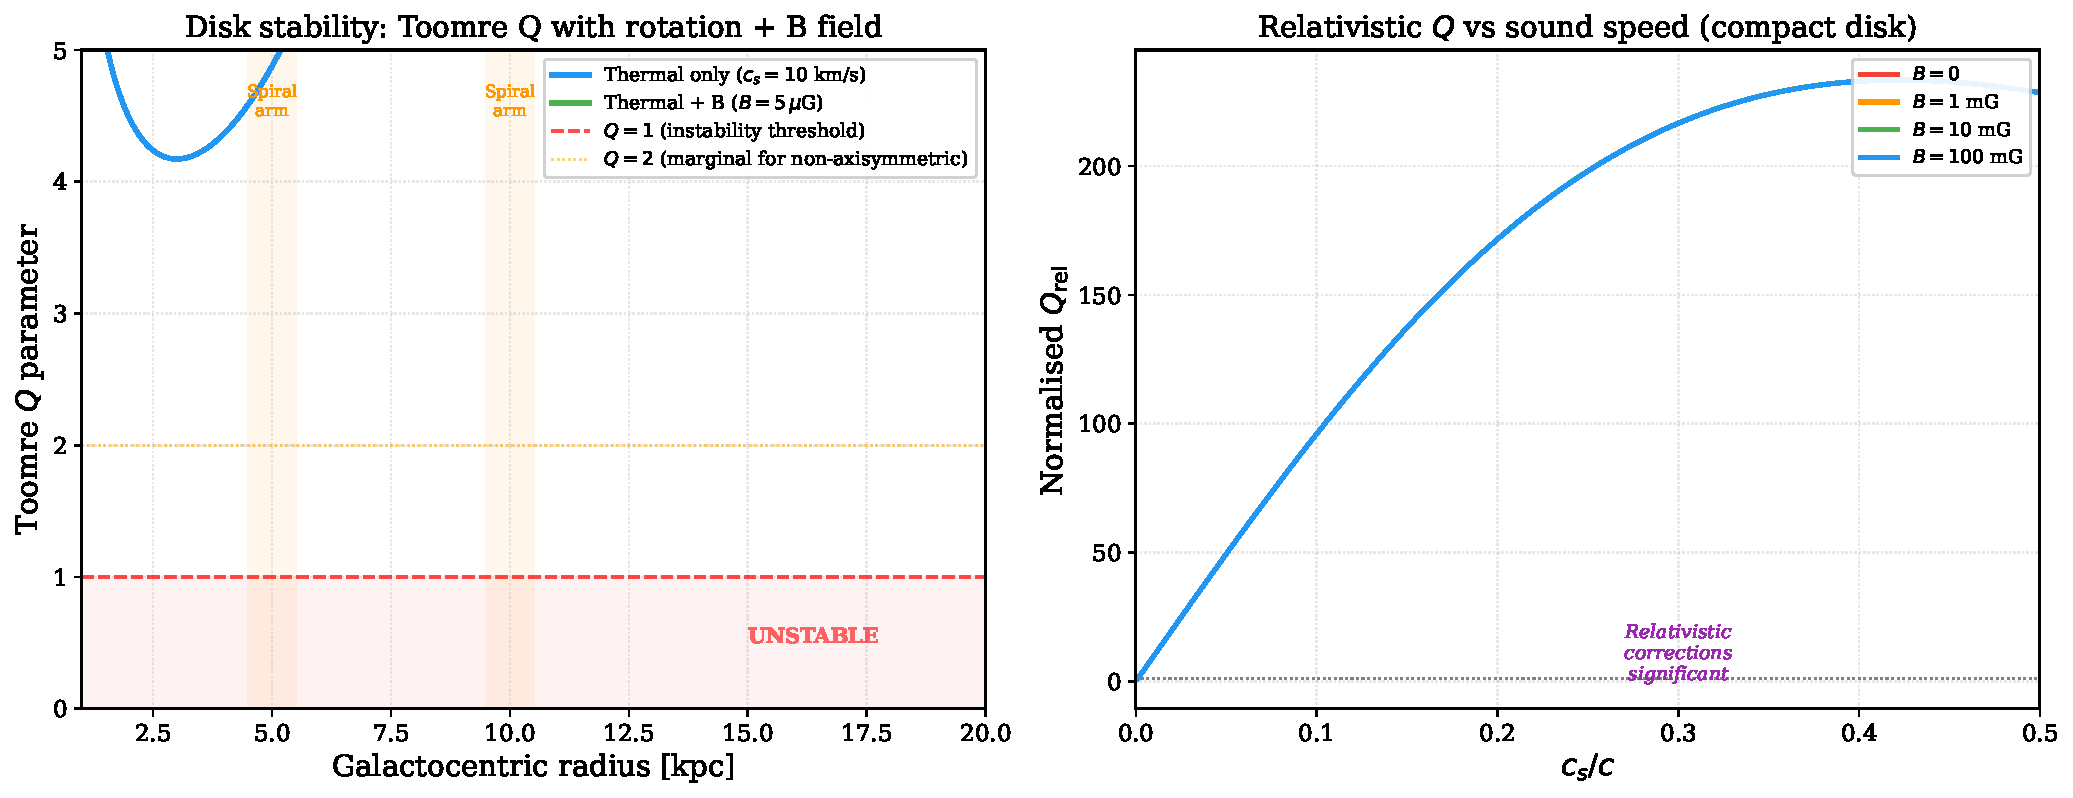
\includegraphics[width=\textwidth]{plots/ch13/fig_toomre_Q_disk.pdf}
\caption{%
  \textbf{Left:} Toomre $Q$ parameter as a function of
  galactocentric radius for a model spiral galaxy with a flat
  rotation curve ($V_{c} = 220$~km/s) and exponential surface
  density profile.  The thermal-only case ($c_{s} = 10$~km/s)
  is compared with the magnetically supported case
  ($B = 5\,\mu$G).  Orange bands mark schematic spiral-arm
  locations where enhanced surface density drives $Q$ down toward
  the instability threshold $Q = 1$.
  \textbf{Right:} Normalised relativistic $Q_{\mathrm{rel}}$ as a
  function of $c_{s}/c$ for different magnetic field strengths in a
  compact disk, showing how relativistic effects (enthalpy
  corrections, bounded $v_{A}$) modify the stability boundary at
  high sound speeds.
}
\label{fig:toomre-Q-disk}
\end{figure}

In the \textbf{Milky Way disk}, the Toomre parameter is typically
$Q \sim 1$--$2$, placing the disk near marginal stability.  Star
formation is concentrated in spiral arms where gas compression
reduces $Q$ toward unity~\citep{Toomre1964,BinneyTremaine2008}.
The magnetic field ($B \sim 5\,\mu$G in the interstellar medium)
provides additional support, raising $Q$ by $\sim 10$--$30\%$, as
shown in the left panel of Figure~\ref{fig:toomre-Q-disk}.

In \textbf{AGN accretion disks}, where the gas temperature and
magnetic field strengths are much higher, relativistic corrections
to $Q$ become significant.  The enthalpy replacement
$\rho \to (\varepsilon + p)/c^{2}$ increases the effective surface
density, while the bounded Alfv\'en speed $v_{A} < c$ limits the
magnetic support.  These effects reduce $Q_{\mathrm{rel}}$ below
the classical value, potentially triggering gravitational
fragmentation in the outer regions of AGN
disks~\citep{RezzollaZanotti2013}.

%------------------------------------------------------------------
\section*{BIBLIOGRAPHICAL NOTES}
\label{sec:rel-120-bib}

The gravitational instability of an infinite homogeneous medium was
discovered by Jeans:

\begin{enumerate}
\item J.~H.~Jeans, `The stability of a spherical nebula',
  \textit{Phil.\ Trans.\ Roy.\ Soc.\ (London)}, \textbf{199}, 1--53
  (1902).
\end{enumerate}

\noindent
The classical effects of rotation and magnetic field on Jeans's
criterion were analysed systematically by Chandrasekhar:

\begin{enumerate}
\setcounter{enumi}{1}
\item S.~Chandrasekhar, `The gravitational instability of an infinite
  homogeneous medium when a Coriolis acceleration is acting',
  \textit{Vistas in Astronomy~I}, 344--7 (1955).
\item S.~Chandrasekhar and E.~Fermi, `Problems of gravitational
  stability in the presence of a magnetic field',
  \textit{Astrophys.\ J.}\ \textbf{118}, 116--41 (1953).
\item S.~Chandrasekhar, `The gravitational instability of an infinite
  homogeneous medium when Coriolis force is acting and a magnetic
  field is present', \textit{Astrophys.\ J.}\ \textbf{119}, 7--9
  (1954).
\end{enumerate}

\noindent
The relativistic treatment of self-gravitating systems in the context of
cosmological perturbation theory was initiated by:

\begin{enumerate}
\setcounter{enumi}{4}
\item H.~Bondi, `Massive spheres in general relativity',
  \textit{Proc.\ Roy.\ Soc.\ (London)}~A, \textbf{282}, 303--17
  (1964).
\item E.~M.~Lifshitz, `On the gravitational stability of the expanding
  universe', \textit{J.\ Phys.\ (USSR)}, \textbf{10}, 116 (1946).
\end{enumerate}

\noindent
The relativistic Jeans analysis in a static background, including the
role of pressure as a gravitational source, is discussed in:

\begin{enumerate}
\setcounter{enumi}{6}
\item S.~Weinberg, \textit{Gravitation and Cosmology}, chap.~15,
  Wiley, 1972.
\item J.~M.~Bardeen, `Gauge-invariant cosmological perturbations',
  \textit{Phys.\ Rev.}~D, \textbf{22}, 1882--905 (1980).
\end{enumerate}

\noindent
Relativistic magnetohydrodynamic stability, including the formulation of
causal MHD with bounded characteristic speeds, is treated in:

\begin{enumerate}
\setcounter{enumi}{8}
\item A.~Lichnerowicz, \textit{Relativistic Hydrodynamics and
  Magnetohydrodynamics}, Benjamin, New York, 1967.
\item K.~S.~Thorne, `Relativistic stellar structure and dynamics',
  in \textit{High Energy Astrophysics} (ed.\ C.~DeWitt, E.~Schatzman,
  P.~V\'eron), Gordon \& Breach, 1967.
\item A.~M.~Anile, \textit{Relativistic Fluids and Magneto-Fluids},
  Cambridge University Press, 1989.
\end{enumerate}

\noindent
The Toomre criterion and its relativistic extension for self-gravitating
discs:

\begin{enumerate}
\setcounter{enumi}{11}
\item A.~Toomre, `On the gravitational stability of a disk of stars',
  \textit{Astrophys.\ J.}\ \textbf{139}, 1217--38 (1964).
\item E.~Rezzolla, O.~Zanotti, \textit{Relativistic Hydrodynamics},
  Oxford University Press, 2013, \S\,11.
\end{enumerate}

\noindent
The review by Pacholczyk and Stodkiewicz on the combined effects of
rotation and magnetic field remains an excellent reference:

\begin{enumerate}
\setcounter{enumi}{13}
\item A.~G.~Pacholczyk and J.~S.~Stodkiewicz, `On the gravitational
  instability of some magnetohydrodynamical systems of astrophysical
  interest', \textit{Acta Astronomica} \textbf{10}, 1--29 (1960).
\end{enumerate}

\noindent
For causal dissipation frameworks ensuring finite propagation speeds in
relativistic fluids, the BDNK first-order theory provides a rigorous
alternative to second-order approaches:

\begin{enumerate}
\setcounter{enumi}{14}
\item F.~S.~Bemfica, M.~M.~Disconzi and J.~Noronha, `Nonlinear
  causality of general first-order relativistic viscous hydrodynamics',
  \textit{Phys.\ Rev.\ D}\ \textbf{98}, 104064 (2018).
\item P.~Kovtun, `First-order relativistic hydrodynamics is stable',
  \textit{JHEP}\ \textbf{10}, 034 (2019).
\item F.~S.~Bemfica, M.~M.~Disconzi and J.~Noronha, `Causality and
  existence of solutions of relativistic viscous fluid dynamics with
  gravity', \textit{Phys.\ Rev.\ D}\ \textbf{107}, 076012 (2023).
\end{enumerate}
